%--------------------------------------------------------------------------
%	PACKAGES AND OTHER DOCUMENT CONFIGURATIONS
%--------------------------------------------------------------------------
\documentclass[11pt,a4paper]{article}
\usepackage[utf8]{inputenc}
\usepackage[english]{babel}
\usepackage[T1]{fontenc}
\usepackage{amsmath}
\usepackage{mathtools}
\usepackage{amsfonts}
\usepackage{amssymb}
\usepackage{pifont}% http://ctan.org/pkg/pifont
\usepackage{graphicx}
\usepackage{epstopdf}
\usepackage{lmodern}
\usepackage[left=3cm,right=3cm,top=2.5cm,bottom=2.5cm]{geometry}

\usepackage{fancyhdr} % Required for custom headers
\usepackage{lastpage} % Required to determine the last page for the footer
\usepackage{extramarks} % Required for headers and footers
%\usepackage[usenames,dvipsnames]{color} % Required for custom colors
\usepackage[usenames,dvipsnames]{xcolor}
\usepackage{graphicx} % Required to insert images
\usepackage{caption}
\usepackage{subcaption}
\usepackage{listings} % Required for insertion of code
%\usepackage{courier} % Required for the courier font
\usepackage{verbatim}
\usepackage{multirow}
\usepackage{eurosym}
\usepackage{url}
\usepackage{hyperref}
\usepackage[outline]{contour}
 \contourlength{.5pt}
\usepackage[noadjust]{cite}
\usepackage{tabularx}

\usepackage{enumerate}
\usepackage{enumitem}
\setlist[itemize]{noitemsep, topsep=0pt, label={---}}
\usepackage{todonotes}
%\usepackage{relsize}

\usepackage{tikz}
\usetikzlibrary{matrix}

\setlength\parindent{0pt} % Removes all indentation from paragraphs
\setlength{\parskip}{5pt plus 1pt minus 1pt}

%\definecolor{bleu}{HTML}{0000FF}
%\definecolor{jaune}{HTML}{EDB601}
%\definecolor{vert}{HTML}{008E45}
%\definecolor{rouge}{HTML}{FF0000}

%\renewcommand\thesection{\Roman{section}}

\providecommand{\e}[1]{\ensuremath{\times 10^{#1}}}

\begin{document}
	
%--------------------------------------------------------------------------
%	TITLE PAGE
%--------------------------------------------------------------------------
\begin{center}
{\bfseries
Linköping University\\
TDDD17 Information Security, Second Course\\

Lab 1: Authentication with OpenID\\
Lab assistant: Ulf Kargén\\[10pt]}

Guillaume Lambert (guila302) and Lena Peschke (lenpe782)\\
version 1, 20-02-27
\end{center}

\hrulefill

%--------------------------------------------------------------------------
%	CONTENT
%--------------------------------------------------------------------------

\section*{Our own authentication method}
\subsection*{Design of an authentication method}
\paragraph{Description}
% design choices

Our authentication method is challenge-response. It is based on a choice of matrix positions, colours and a password made at the registration.
These choices determine the answer to the challenges that are sent by the server to the user.

More concretely the challenge consists of a randomly generated $3\times3$-matrix in which each of the 9 positions may contain a different letter and colour.
The answer the user has to provide is made of the letters that fit his choices by either being in the right position inside the matrix, of the right colour, or simply a letter contained in the password. The user thus has to identify the components that overlap with his personal secret.

If no letters fit at least one of the chosen characteristics the entire password has to be entered.

If the user enters the wrong response, a new matrix is generated and he has the chance to try again. We decided not to limit the number of tries in this system.

The parameters among which the user has to choose are:
\begin{itemize}
\item 3 to 7 matrix positions (among 9)
\item 2 to 4 colours among 6 (black, brown, blue, red, green, purple)
\item a password of maximum 12 letters but with at least 4 different letters. Case is not considered.
\end{itemize}

\textit{Example:} A user chooses the following scheme.
\begin{itemize}
\item matrix positions: $(1,3) (2,3) (3,2) (3,3)$
\item colours: \textcolor{blue}{blue} \textcolor{ForestGreen}{green} \textcolor{RoyalPurple}{purple}
\item password: \texttt{password}
\end{itemize}
When presented with a randomly generated challenge as presented in Figure~\ref{fig:ex1}, the user has to select the squares containing A, I, and X. His answer will be \texttt{xia} (in this order).
\begin{figure}[!ht]
\centering
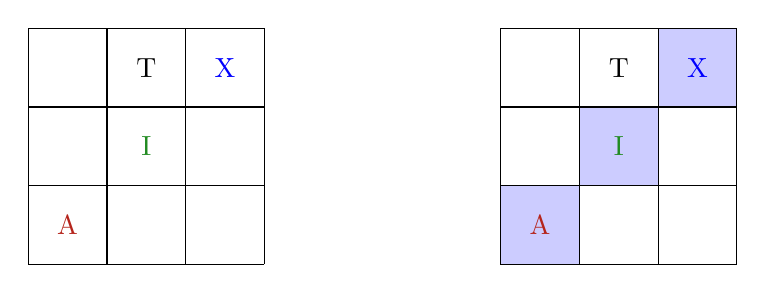
\begin{tikzpicture}
\draw[step=1cm,color=black,thin] (0,0) grid (3,3);
\node[BrickRed] at (0.5,0.5) {A};
\node[black] at (1.5,2.5) {T};
\node[ForestGreen] at (1.5,1.5) {I};
\node[blue] at (2.5,2.5) {X};

\draw[step=1cm,color=black,thin] (6,0) grid (9,3);
\filldraw[fill=blue!20!white, draw=black] (6,0) rectangle (7,1);
\filldraw[fill=blue!20!white, draw=black] (7,1) rectangle (8,2);
\filldraw[fill=blue!20!white, draw=black] (8,2) rectangle (9,3);
\node[BrickRed] at (6.5,0.5) {A};
\node[black] at (7.5,2.5) {T};
\node[ForestGreen] at (7.5,1.5) {I};
\node[blue] at (8.5,2.5) {X};
\end{tikzpicture}
\caption{Example of a challenge-response. The left matrix is the challenge and the right the response, where the blue squares are the ones selected by the user.}
\label{fig:ex1}
\end{figure}

\paragraph{Risk analysis} We chose to draw an attack tree as a risk analysis of our authentication method. The attack goal is to access the chat without a valid account. The entire tree is represented in Figure~\ref{fig:attacktree}.
\begin{figure}[!ht]
\centering
\includegraphics[width=1\textwidth]{attacktree.pdf}
\caption{Attack tree of our own authentication method.}
\label{fig:attacktree}
\end{figure}
We used the labels \textcolor{ForestGreen}{Possible} and \textcolor{BrickRed}{Impossible}, making the assumption that the chat RP, the OpenID OP and the users are on separate machines and servers. We did not use cost or probability estimates, because these would highly depend on the actual use of the system.
The tree contains the major threats we were able to identify for the system. We divided them into two main categories: getting a login or cracking the system.
Two particular items need some explanation.
\begin{itemize}
\item All the possibilities in the subtree \texttt{Log in to chat $\rightarrow$ Get login $+$ password $\rightarrow$ From machine} are labeled as impossible. Spying on the screen or using a key logger once do not reveal the secret, as each challenge requires a customised response. They become possible however if used repeatedly until a statistical analysis of the data makes it possible to deduce the secret. The impossible label in this case stands for an effort we have estimated as too time consuming as it would only reveal a single login. The database is different as it contains all accounts. We have added the leaf \texttt{Decrypt DB} although it is not encrypted as it is now; because the risk analysis comes to the conclusion that accessing it is already impossible, encrypting it is not needed to make an attack impossible, which is why it can leave it unencrypted for now.
\item The dictionary attack in the subtree \texttt{Log in to chat $\rightarrow$ Crack the system $\rightarrow$ Guess password} is labeled as impossible for the same reason as mentioned above: it would require a lot of time due to the repetitions that are necessary to gather useful statistical data. Every password has to be used enough times to make sure that it does never grant access to a given user account. This effect is however somewhat limited by the fixed maximum length of the password.
\end{itemize}

As we can see in the tree, the final conclusion is that an intrusion is possible both by acquiring a login and password and by cracking the system. As in most authentication systems, the user itself is a major security threat. We identified bribing and asking (with some social engineering) as the main threats which involve human users. The second major threat is the backdoor.
We concluded that SQL injection and eavesdropping on the network are both possible. Several methods can mitigate SQL injections: prepared statements and restricted permissions have proven efficient. Despite these measures, we still think of the attack as possible because it primarily concerns our way of handling the database, which may be error-prone.
The replay attack seems possible to us due to the lack of tokens in the communication between the user and the OpenID OP.

\paragraph{Security of our method}
Our method is based on a challenge-response scheme in which the server and the user have to ``compute'' the response separately.
Compared to passwords, the information exchanged between the two parties is less likely to give away the secret: each challenge expects a different response that depends on the user.
An intruder trying to steal a user's secret based on what the user sends to the server needs patience: he has to eavesdrop for a long time before he can try to recover the password, the matrix positions and the colours based on the user's different responses to different challenges. For each response, an entered letter can be a part of the matrix, the colour or the letter secret component, as well as belonging to several among them.
If the intruder has access to the challenge, which is sent as a picture from the server, he can work faster by excluding all the non-selected positions.

The security provided through the storage at a the server side is comparable to passwords, as the secret also has to be stored in a database.

Number of possible secrets:
$$ \sum\limits_{p=3}^{7}{9 \choose p} +  \sum\limits_{c=2}^{4}{6 \choose c} + \sum\limits_{l=4}^{12}{26 \choose k} = 646 406 904 000 \approx 6.5\e{11}$$

Number of possible challenge matrices:\todo{CHECK MATH!!!}
$$ 2 \times {6 \choose 1} \times {26 \choose 1} \times \sum\limits_{p=3}^{6}\left[{p\times {9 \choose p}}\right] = 589680 \approx 5.9\e{5}$$

\paragraph{Use-case diagram} The use case diagram of our authentication mechanism, represented in Figure~\ref{fig:usecasedia}, depicts the interactions between the user and the system. It does not take the OpenID mechanism into account and only deals with plain authentication, thus not representing further functionalities.
\begin{figure}
\centering
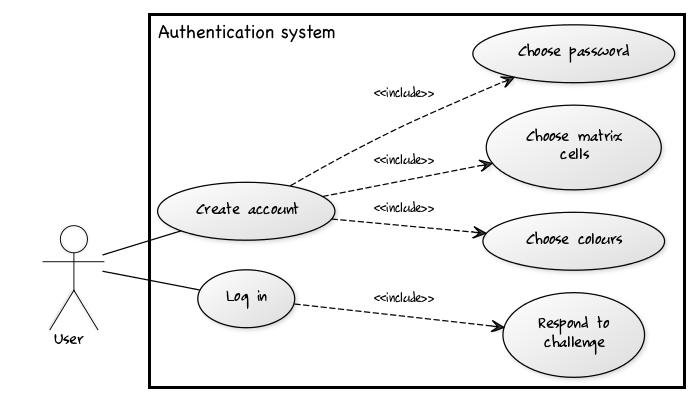
\includegraphics[width=0.9\textwidth]{usecasedia.png}
\caption{Use case diagram of our authentication method [created with \url{www.yuml.me}].}
\label{fig:usecasedia}
\end{figure}


\paragraph{Sequence diagram} The sequence diagram of our authentication mechanism is represented in Figure~\ref{fig:seqdia}. We do not consider the OpenID mechanism in it.
\begin{figure}
\centering
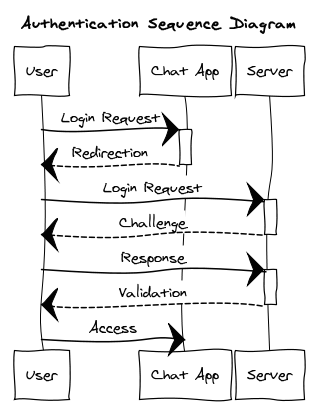
\includegraphics[width=0.6\textwidth]{seqdia.png}
\caption{Sequence diagram of our authentication method [created with \url{www.websequencediagrams.com}].}
\label{fig:seqdia}
\end{figure}

\clearpage

\subsection*{Implementation of an authentication method}
\paragraph{Overview}
Our authentication method needs changes in nearly every aspect of the code. The biggest difference to a password authentication is that there are 4 exchanged messages between the user and the server instead of 2, as can be seen in the sequence diagramme (Figure~\ref{fig:seqdia}). Previously, the user would send his username and password to the server, which would either grant or refuse access. With our method, the user sends his username, the server generates a challenge, remembers the expected answer and sends out the matrix to the user. The user then sends his answer and username back to the server, which again grants or refuses access. This impacts the database, the interface and the network aspect of the authentication.

\paragraph{Database}
The table \texttt{OPUserTable} needs to be changed in the database.
An attribute that contains the selected matrix positions and another one for the selected colours need to be added to remember the users credentials.
An additional attribute has to be there: the expected response value. Once the server issues a challenge, it has to remember what response a given user should send back next. This is stored and deleted as soon as a response from the user is received, whether correct or not, as in both cases the next challenge will be a new one.

The requests to the database change as well: instead of retrieving the password of a user for login, the system has to solve a challenge for the user by accessing his entire secret and comparing it to the newly generated challenge.

\paragraph{User interface, HTML and CSS}
As mentioned previously, the authentication is performed in four steps:
\begin{itemize}
\item The user can enter a username;
\item the server generates a challenge and presents it to the user;
\item the user enters his response;
\item the server checks the response and either redirects the user or denies access.
\end{itemize}
The first ``Login''-section will only have a username field. We remove the password field from the original page.  When the username is submitted, another page with the challenge image and an answer field will appear. This is handled in the script \texttt{OPLogin.js}. Once the answer to the challenge is entered correctly, the current user page will appear and the application will continue as it is now.

For signup, the user has to enter matrix positions, colours and a password; these fields need to be added to the ``Create Account''-section.

We also added some explanations on how to use the system to the left of the page.

Finally, a little CSS was added for the instructions text and the challenge image.

\paragraph{Servlets}
A new servlet, \texttt{OPChallengeGenerator}, is to be added. It gets the entered username, sent with a POST request, and handles the GET request for the new page. It generates the challenge and then uses the previously received username as input for calculating the expected answer. It calls the database to store it and sends out the challenge image as a response to the request.
The answer to the challenge entered by the user is handled by \texttt{OPLoginHandler} as previously, but with an adapted validation method.

\texttt{OPCreateUserHandler} needs some modifications too. Upon submission of the form by the user, it has to check all the input to determine if it meets the requirements before storing the new user in the database.

\paragraph{OpenIDA}
In addition to the changes already described above, we needed some new files:
\begin{description}
\item[\texttt{User.java}] This class represents a user and is used to simplify the challenge solving when the user secret is retrieved from the database.
\item[\texttt{UserNotFoundException.java}] In addition to the whole error handling, this exception covers the specific case when a username was not found in the database.
\item[\texttt{UserSecretHandler.java}] This class contains static methods used to convert the user information stored in the database to the types used in the \texttt{User}, which are easier to handle but not easy to store with SQL.
\item[\texttt{Challenge.java}] Located in a subpackage of \texttt{openidProviderPackage}, this class represents a challenge including methods to generate it randomly and to solve it for any user.
\item[\texttt{Square.java}] Located in a subpackage of \texttt{openidProviderPackage}, this class is used by
\texttt{Challenge} and represents a single matrix position.
\item[\texttt{Drawer.java}] Located in a subpackage of \texttt{openidProviderPackage}, this class is used to draw a visual representation of the challenge, as is then presented to the user.

\end{description}

\paragraph{Security flaws}
We found two security flaws in the main implementation.
\begin{itemize}
\item The passwords (and our answers) are sent in clear text in the HTTP messages and stored in clear in the database. When dealing with passwords, an eavesdropper can just read all the information he needs from the intercepted messages and steal the user's identity. The same applies to a database: once an intruder gets access to it, it can read out all usernames and associated passwords. This vulnerability can be prevented with encryption in the database and the messages. The sensible data sent over the network could for instance be hashed.
\item A replay attack between the user and OpenIDA is possible. If an eavesdropper gets ahold of the authentication message sent by the user to the server, it can send it against to masquerade as the user. A countermeasure to this attack are tokens to make messages unique. With our authentication method, the replay is less effective because a new challenge is generated at each login attempt and because the expected answer is deleted from the database as soon as it is retrieved for comparison. Nevertheless, it remains possible because the server does not perform the entire authentication atomically.
\end{itemize}

\end{document}
